\chapter{Conclusiones}
\label{chap:conclusiones}

Aunque el sistema que hemos desarrollado, en concreto, no sirva para resolver ningún problema real (la ubicación en base a la temperatura no es un sistema fiable de posicionamiento), nuestro modelo sí que cumple con las características de un modelo real (en concreto, de machine learning) implementado con criptografía homomórfica:

\begin{itemize}
    \item Un sistema de generación de modelo lento, que sólo se tiene que ejecutar una vez
    \item Otro sistema rápido de evaluación de datos, que se ejecuta múltiples veces
\end{itemize}

Esto nos permite extraer conclusiones acerca de la viabilidad del uso de librerías de criptografía homomórfica en procesos reales:

\begin{enumerate}
    \item El problema de la eficiencia es un problema realmente grave para aplicarlo a sistemas reales: por mucho que optimizásemos nuestra solución, los $50$ ms que tarda en calcularse la curva de regresión en \textit{python} (un lenguaje que ya de por sí es lento comparado con los lenguajes compilados) equivalen a ejecutar dos puertas lógicas de TFHE.
    \item Independientemente de la eficiencia, es difícil programar soluciones con estas librerías, que funcionen, y que realmente sean seguras. Hay que saber mucho para hacerlo correctamente, y se pueden cometer errores que comprometan seriamente la seguridad (\cite{peng_danger_2019}).
\end{enumerate}

Sin embargo, existen ciertos aspectos esperanzadores en todo el asunto. Es muy buena idea en TFHE que limiten los parámetros a elegir. El desarrollador debe poder trabajar con las librerías de forma segura sin tener que elegir los parámetros o comprender qué hacen (eso debe ser trabajo de los criptógrafos).

Como hemos visto a lo largo del máster, en un ámbito profesional las medidas de seguridad tienen que implementarse en función del riesgo del sistema. Estas librerías pueden ser útiles, por ejemplo, para operaciones extremadamente confidenciales que tengan que ser ejecutadas en nubes públicas, siempre que el valor del activo así lo requiera (en comparación con el coste de desarrollar la solución, y el coste computacional extra).

En el estadío actual de las implementaciones de criptografía homomórfica no hay una solución clara que sirva para cualquier problema. Lo ideal es buscar dicha solución para cada caso concreto. Si bien esto puede incrementar el coste (es difícil reutilizar código), hace que el uso de criptografía homomórfica sea viable. Por ejemplo, mientras que nuestra solución pretende ser muy versátil para experimentar con las tecnologías, si se va a trabajar con 64 bits es mucho más eficiente implementar las operaciones en circuitos cerrados de 64 bits (como se haría en un circuito físico).

En cualquier caso, estas tecnologías prometen ser la solución a varios problemas: además de la criptografía homomórfica, la criptografía basada en \textit{lattices} es una de las aproximaciones más prometedoras en un panorama \textit{post-quantum}.

En su presentación en el año 2016, los desarrolladores de TFHE aceptaron un reto: crear sistemas FHE prácticos en menos de 10 años (figura \ref{fig:tfhe_challenge_accepted}, (\cite{chillotti_tfhe:_2016})). Los experimentos que hemos realizado con sus tecnologías, y los trabajos futuros con las tecnologías más recientes, muestran visos de optimismo.

\begin{figure}[h]
    \centering
    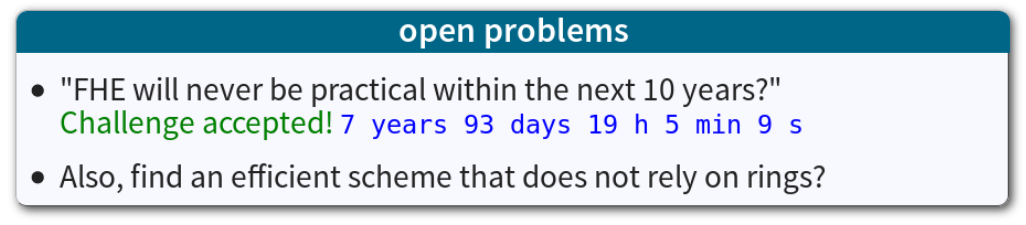
\includegraphics[width=\textwidth]{tfhe_challenge_accepted}
    \caption{``FHE will never be practical within the next 10 years?''}
    \label{fig:tfhe_challenge_accepted}
\end{figure}
